
\chapter{Single Tweet's Creditability Scoring Model} % (fold)
\label{cha:single_tweet_creditbility_scoring_model}
\section{Introduction} % (fold)
At the beginning of an event, the tweets' volume are limited and there is no clear propagation pattern yet. So same as the method of human verifying rumors we can only focus on the information from each single tweet. Therefore, a single tweet classification model can help us detect the rumors on the early stage. 


\section{Motivation and Related Work} % (fold)

Most of the pervious research focus on event level rumors and claim that the task of classification for individual tweet is not reliable \cite{liu2015real} \cite{ma2015detect} \cite{zhao2015enquiring}, because a single tweet is too short to contain enough features. But Carlos Castillo et al. designed a single tweet's creditability rank system: Tweetcred \cite{gupta2014tweetcred}. So we think it is still enable to build up a single tweet's creditability scoring model. 

Recently deep learning is new technology which is used in various areas. And we are inspired by the work of J Ma et al. \cite{lai2015recurrent} that we may use neural network without handcrafted features to build up the single tweet's creditability model which in later experiments outputs a better performance.  
   Zhou et al. invented a C-LSTM model \cite{zhou2015c} for short text classification. The architecture of the model is shown in Figure \ref{fig:CNNLSTMde}. Front hidden layer is a CNN which can split the text into different feature sets and the pooling layer groups the same types of feature together. The last hidden layer is a LSTM layer. They test the model with sentiment classification of  comments on IMDb website. According to his paper, C-LSTM achieved the best result for a 2-classification task with 87.8\% accuracy. We adapt their work to our rumor detection task.

  

\section{Features}
\label{featuressingle}
In this section, we will introduce the features which we use for single tweet's credibility score model. We use a collection of features majorly from Castillo's Tweetcred system \cite{gupta2014tweetcred} with totally 27 features shown in Table \ref{tab:single_features}. These features can be extracted directly from Twitter interface without third part website. 
\subsection{Text Features}
The Text features capture the content of tweets. There are 16 Text features like the length of the tweets. 
\textbf{Sentiment Features} are included in text features.
We used the python natural language Toolkit (nlTK)\footnote{http://www.nltk.org/} to analyze the tweets' sentiment and extract the features: the \emph{NumPositiveWords}, \emph{NumNegativeWords} and \emph{PolarityScores}. \emph{PolarityScores} is a float for sentiment strength of one tweet\footnote{http://www.nltk.org/api/nltk.sentiment.html} $Polarity\_scores = \frac {1}{N}    \sum_{0}^{n} {Polarity(token_n)}$.

\subsection{User Features} We selected total 6 features of the posters. These features are extracted directly from the Twitter interface as in Figure \ref{fig:UserSample}. ReputationScore is defined as the ratio between \#Friends over \# Followers. $ReputationScore = \frac {\#Friends }{\#Friends +\#Followers}$.
\begin{figure}[!h]
\centering
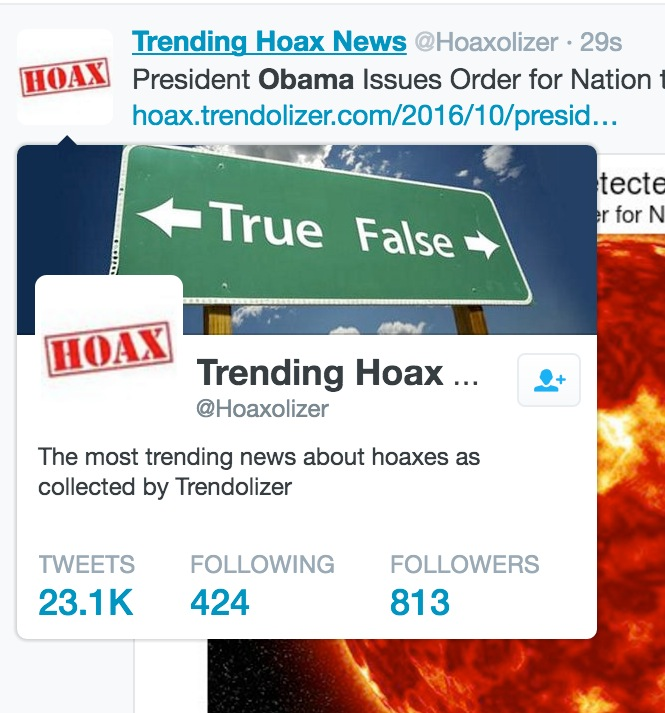
\includegraphics[width=0.45\columnwidth]{images/UserSample.png}
\caption{Sample of Users' Information on Twitter Interface}
\label{fig:UserSample}
\end{figure}
\newpage
\subsection{Twitter Features} Twitter Features are the features which are extracted from the unique functions of Twitter website. It includes \emph{hashtag}, \emph{mention}, \emph{number of URLs}, \emph{number of retweets} and whether this tweet is \emph{retweet} (contains RT as keywords).


\begin{table*}[!h]
\small
\centering
\scalebox{0.8}{
 \begin{tabular}{@{}lllllll@{}}
 \toprule
 \textbf{Category} & \textbf{Feature} & \textbf{Description}\\ \midrule
 Twitter Features& Hashtag & Whether the tweet contains \#hashtag\\
 		& Mention & Whether the tweet mentions others @user\\
 		& NumUrls & \# url in the tweet \\
 		& Retweets & How many times this tweet has been retweeted \\ 
 		& IsRetweet & Whether this tweet is retweeted from others\\
\midrule
 Text Features & LengthOfTweet & The length of tweet\\
    & NumOfChar & \# of individual characters \\
   & Capital &  Fraction of characters in Uppercase \\
   & Smile & Whether this tweet contains :->, :-), ;->, ;-)\\
   & Sad & Whether this tweet contains :-<, :-(, ;->, ;-(\\
   & NumPositiveWords & \# of positive words\\
   & NumNegativeWords & \# of negative words\\
   & PolarityScores & polarity scores of the Tweet\\
   & Via & Whether this tweet contains via\\
   & Stock & Whether this tweet contains \$ \\
   & Question & Whether this tweet contains ? \\
   & Exclamation & Whether this tweet contains ! \\
   & QuestionExclamation & Whether this tweet contains multi Question or Exclamation mark \\ 
   & I & Whether this tweet contains  first pronoun like I, my, mine, we, our   \\
   & You & Whether this tweet contains second pronoun like U, you, your, yours \\ 
   & HeShe & Whether this tweet contains third pronoun like he, she, they, his, etc. \\\midrule
   User Features & UserFollowers  & \# of followers\\
 	& UserFriends  & \# of friends\\
 	& UserTweets  & \# of tweets which are posted by this user\\
 	& UserDescription  & Whether this user has description\\
 	& UserVerified  & Whether this user is a verified user\\
 	& UserReputationScore & Ratio between \#Friends over (\# Followers + \#Friends)\\
 \bottomrule
 \end{tabular}}
 \caption{Features for Single Tweet's Creditability Scoring Model}
 \label{tab:single_features}
\end{table*}
\clearpage
\section{Experimental Evaluation} % (fold)
  \subsection{Datasets} 
  \label{sec:dataset_single}
In this section, we will introduce the dataset for training and the approach of definition time period of event. We collected rumor stories from a rumor tracking website \textbf{snopes.com} and \textbf{urbanlegends.about.com}. We crawled 4300 stories from the website and we manually constructed 130 queries of them. The approach of constructing queries is mainly following the work \cite{gupta2014tweetcred}. The regular expression of a query is:

 \textbf{ (Object \& Subject \& Description(Description1||Description2||...)) }


For example: a rumor story is about Obama removing a flag in pearl harbor. The first term of regular expression  \emph{"Object"} is  \emph{"Obama"}. The second term  \emph{"Subject"} is  \emph{"flag"} and its synonym:  \emph{flags, flagpole}. The third term  \emph{"Description"} is the keyword "remove" and its synonym:  \emph{removes},  \emph{removing} or a URL link about this rumor like  \emph{"Departed.co"}. In this example, the proper noun \emph{"pearl harbor"} is also necessary. Finally we transform the regular expression:
 
 \textbf{ (Obama \& (flag||flags||flagpole) \& (remove||removal|| removing|| "Departed.co") \& "pearl harbor" ) }
 
into Twitter's query: 

\textbf{Obama (flag OR flags OR flagpole) (remove OR removing OR removal OR "Departed.co") pearl harbor}


%to do %
Pervious works like Liu et al.~\cite{liu2015real} use the news which are reported on \textbf{snopes.com} as the training set. But after we test them, we think these news events contain too less tweets. So we use the dataset from the work of Mcminn et al.~\cite{mcminn2013building}. They crawl tweets with the Twitter Streaming API  from 10th of October 2012 to 7th of November 2012. These events are manually checked that they really happened. From those dataset, we select the top 90 events with most tweets' volume and we add other 40 news events which happened near the time points of rumors. The detail of tweets' volume is shown in Table \ref{tab:Tweet_Volume}:
\begin{table*}[!h]
 \centering
\scalebox{0.8}{
 \begin{tabular}{@{}cccccc@{}}
 \toprule
 \textbf{Type} & \textbf{Min Tweet Volume} & \textbf{Max Tweet Volume}& \textbf{Total Tweet Number} &\textbf{Average Tweet Number} \\ \midrule
 News & 18 & 17414 & 172616 & 1327.82 \\ \midrule
 Rumors & 44  & 26010& 91268 & 702.06\\
 	 \bottomrule
 \end{tabular}}
 \caption{Tweet Volume of News and Rumors}
 \label{tab:Tweet_Volume}
\end{table*}

As we mentioned in the Section \ref{tapi}, the Twitter limits the result of its API by only returning a sample of tweets in recent 7 days. So we have to crawl the data from the web interface. We use Beautiful Soup as the html parsing library to parse the Twitter timeline pages and the users' homepage\footnote{https://www.crummy.com/software/BeautifulSoup/bs4/doc/}. Beautiful Soup is a Python library for pulling data out of HTML and XML files. For increasing the speed of parsing html and extracting features from raw data, we use Spark\footnote{http://spark.apache.org/} technology, because it can simply manage multithread and its mapReduce in memory technology makes the process much faster. 

 After we crawled and parsed the whole timeline of an event, we detected the 48 hours time period of the burst in the way which we will mention in following Section \ref{sec:Time_Period_of_an_Event}. We crawl the homepage of users within the event time period, totally 133,396 users.
 
  \subsubsection{Time Period of an Event}
\label{sec:Time_Period_of_an_Event}

In this section, we will introduce the novel approach of defining the time period of event on Twitter. The time period of a rumor event is hard to define. To the best of our knowledge, there is no related work which gave us an approach about how to define the time period of one rumor event. One reason is a rumor may be created serval years ago and kept exiting in Twitter, but it did not attract the crowd's attention. However it can be triggered by other events after a uncertain time and suddenly quickly spread as a bursty event.

For example, a rumor\footnote{http://www.snopes.com/robert-byrd-kkk-photo/} claimed that Robert Byrd was member of KKK. This rumor has been circulating in Internet for a while, as shown in Figure \ref{fig:KKK_full} that almost every day there were several tweets talking about this rumor. But this rumor was triggered by a picture about Robert Byrd kissing Hillary Clinton in 2016 and twitter users suddenly noticed this rumor and it was spread burstly. And what we are really interested is the tweets which are posted in hours around the bursty peak.
 
\begin{figure}[!h]
\centering
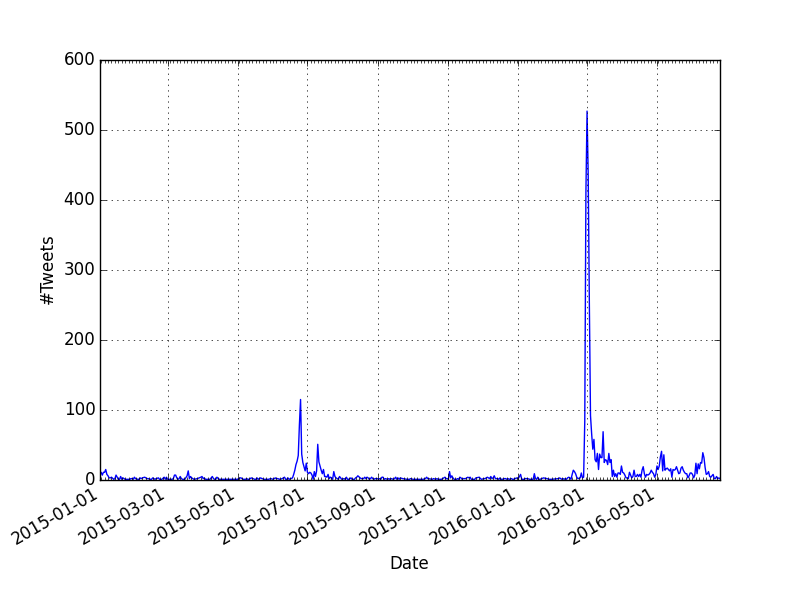
\includegraphics[width=0.7\columnwidth]{images/KKK_figure.png}
\caption{Full Scale Tweets' Volume of Event Robert Byrd}
\label{fig:KKK_full}
\end{figure}

 We defined the hour with the most tweets' volume as $t_{max}$ and we want to detect the rumor event as soon as possible before its burst, so we define the time of the first tweet before $t_{max}$ within 48 hours as the beginning of this rumor event, marked as $t_{0}$. And the end time of events we defined as $t_{end}=t_0+48$. We show the tweets' volume in Figure \ref{fig:KKK_part} of the above rumor events after defined 48 hours time period.
  
\begin{figure}[!h]
\centering
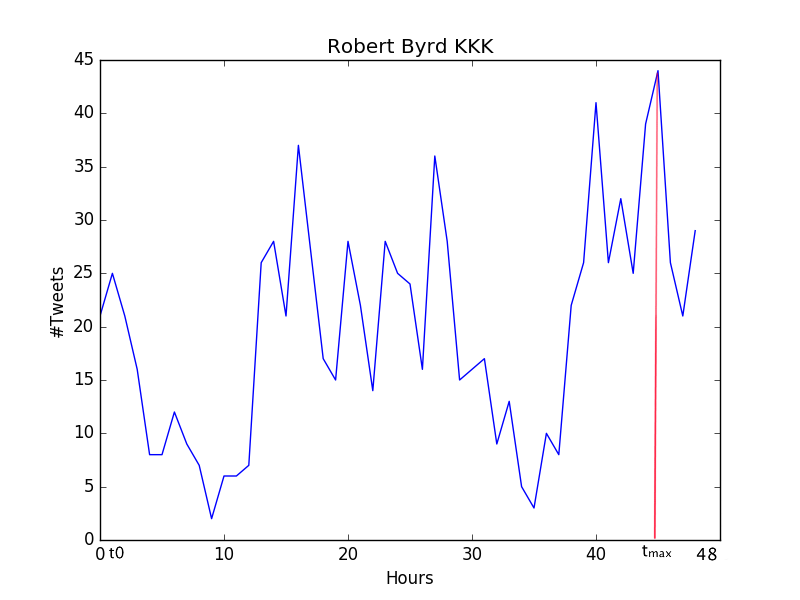
\includegraphics[width=0.7\columnwidth]{images/Robert_Byrd_KKK.png}
\caption{Tweets' Volume of the Rumor Event of Robert Byrd with the Selected Time Period}
\label{fig:KKK_part}
\end{figure}
\newpage
\subsection{Classification Models} % (fold)
In this section, we will introduce the classifiers of single tweet's credibility model. We developed two kinds of classification models: traditional classifier with handcraft features and neural network without handcraft features.
\subsubsection{Single Tweet's Creditability Model with handcrafted features} % (fold)
We follow Castillo's \cite{gupta2014tweetcred} idea to implement a single tweet's creditability model with above handcrafted features in Section \ref{featuressingle}. We select the most popular classification models for testing: decision trees, decision forest and SVM.  

  \subsubsection{Single Tweet's Creditability Model without handcrafted features} 
\label{sec:single_nofeature}

 Inspired by the works of Lai et al. \cite{lai2015recurrent} and J Ma et al.  \cite{madetecting}, we test neural networks as the classifier which does not need to extract features from the data. Based on the previous works, we test 6 models: Basic tanh-RNN \ref{fig:SRNN} as baseline, 1-layer GRU-RNN \ref{fig:1GRU} ,1-layer LSTM \ref{fig:1LSTM}, 2-layer GRU-RNN \ref{fig:2GRU}, FastText \ref{fig:fasttext} and CNN+LSTM \ref{fig:CNNLSTM}  model  as Figure \ref{fig:2GRU} model. Basic tanh-RNN, 1-layer GRU-RNN, 1-layer LSTM-RNN and 2-layer GRU-RNN models are based on the work of J Ma et al. \cite{madetecting}. FastText comes from work  joulin et al.~\cite{joulin2016bag} which is a fast text classification model and FastText dose not need GPU for acceleration. The hybrid model of CNN and LSTM (C-LSTM) is an idea from Zhou et al. \cite{zhou2015c} which has the best performance in our experiments. Zhou et al. test their C-LSTM for sentiment classification by using the dataset of real comments on IMDb website. Those comments are short texts which are similar to tweets and get the best accuracy 86\%. And we adapt their model to our work.

\begin{figure}[]

  \centering

\subfigure[Sample RNN Model]{\label{fig:SRNN}
\centering
  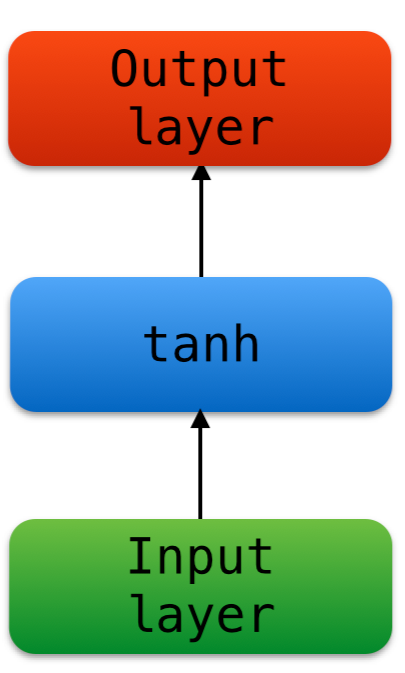
\includegraphics[width=0.22\columnwidth]{images/simRNN.png}
} %
\subfigure[1-layer GRU-RNN]{\label{fig:1GRU}
\centering
  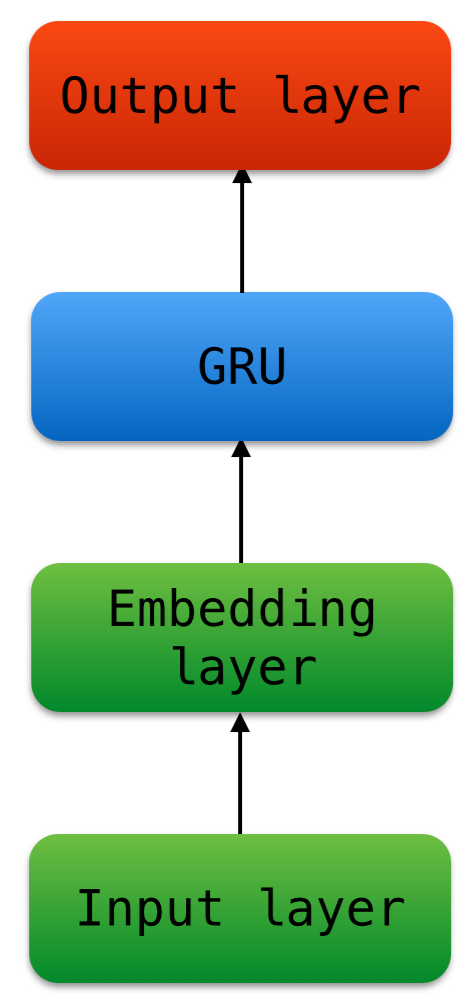
\includegraphics[width=0.22\columnwidth]{images/GRUlayer.png}
}
\subfigure[1-layer LSTM-RNN]{\label{fig:1LSTM}
\centering
  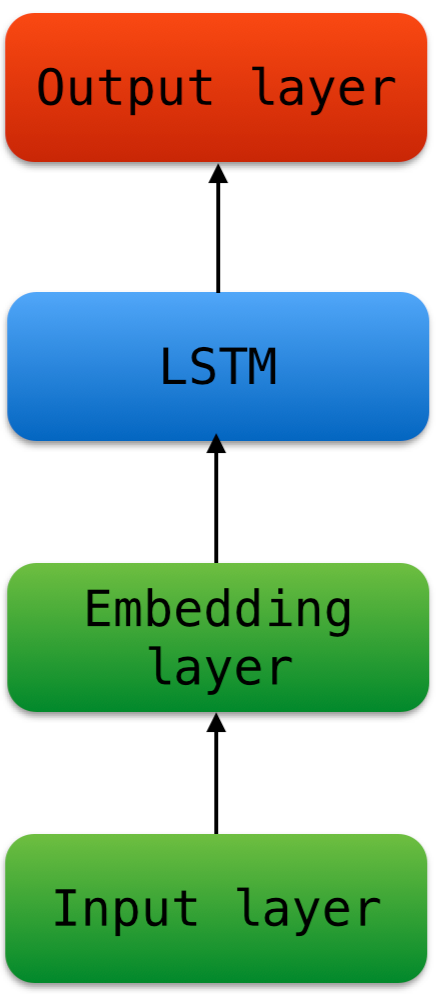
\includegraphics[width=0.22\columnwidth]{images/LSTMLayer.png}
}
\subfigure[2-layer GRU-RNN]{\label{fig:2GRU}
\centering
  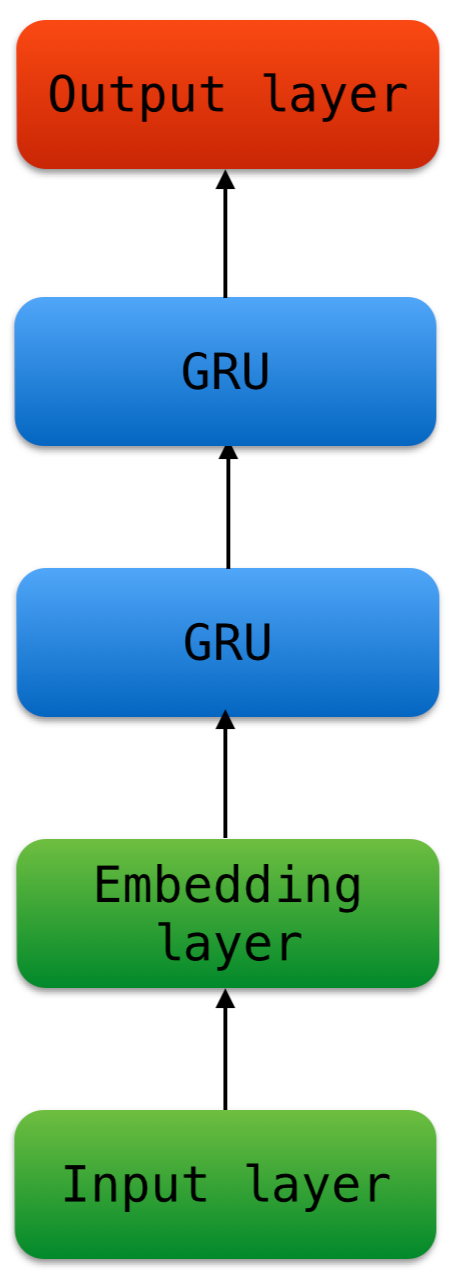
\includegraphics[width=0.22\columnwidth]{images/2gru.png}
}
\subfigure[FastText]{\label{fig:fasttext}
\centering
  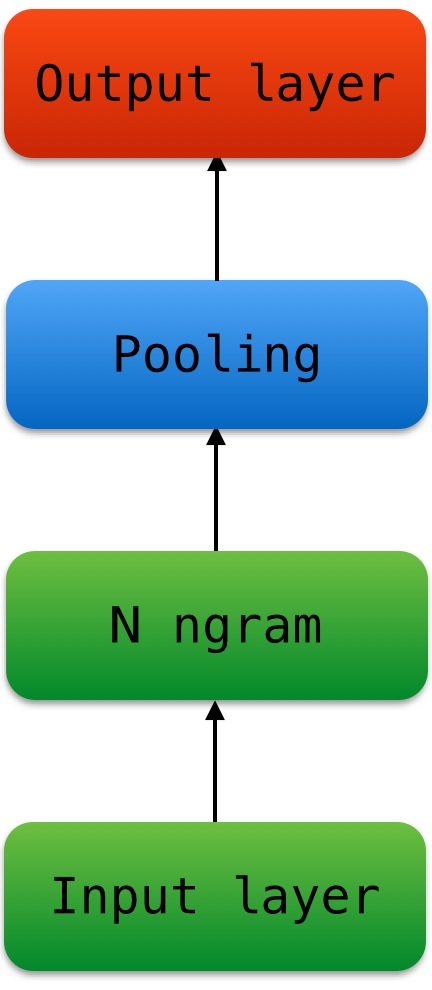
\includegraphics[width=0.22\columnwidth]{images/fasttext.png}
}
\subfigure[Hybrid CNN + LSTM (C-LSTM)]{\label{fig:CNNLSTM}
\centering
  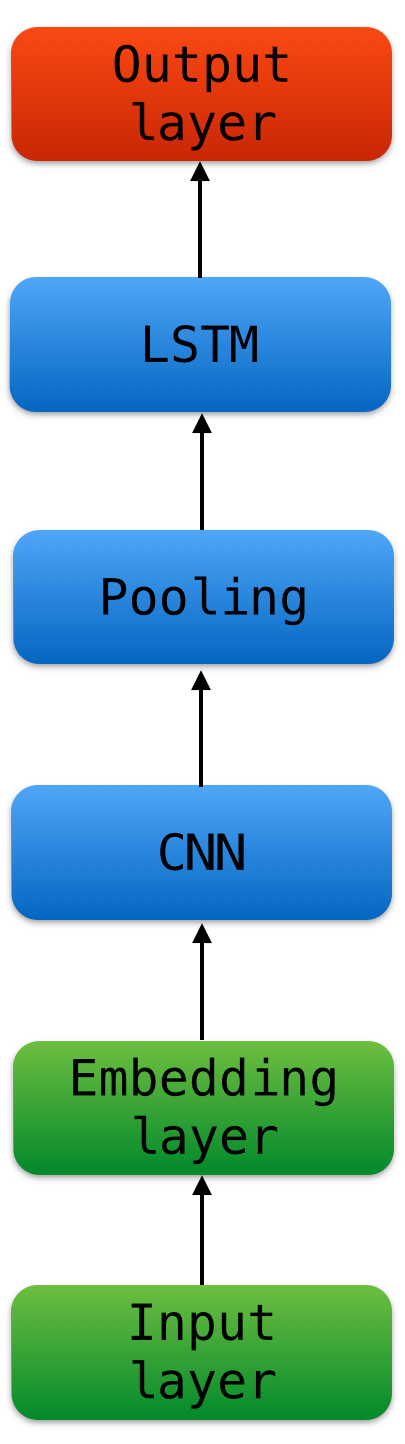
\includegraphics[width=0.22\columnwidth]{images/CNNLSTM.png}
}
\caption{Neural Network Model for Single Tweet Classification}
\label{fig:NNModel1}
\end{figure}

  \begin{figure}
\centering
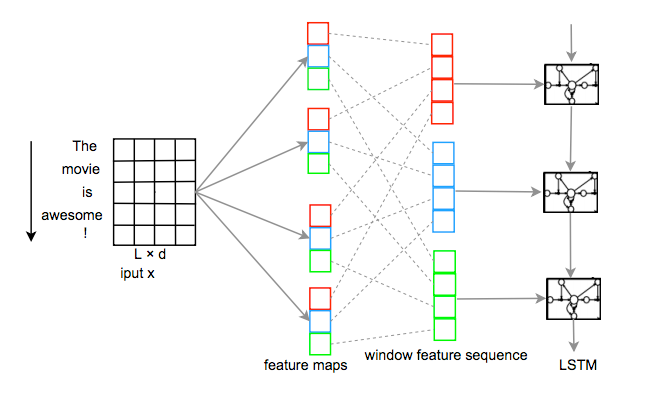
\includegraphics[width=0.8\columnwidth]{images/CNNLSTMdetail.png}
\caption{The Architecture of C-LSTM Interface (source: \cite{zhou2015c})}
\label{fig:CNNLSTMde}
\end{figure} 


\subsection{Experiment Setting}
In this section, we will introduce the experiment setting of single tweet's credibility model. We shuffle the 260 events and split them into 10 subsets which are used for 10 times cross-validation. We show the parameters after optimization for each model in Table \ref{tab:single_model_para}. And we implement these 3 non-neural network models with scikit-learn library\footnote{scikit-learn.org/}. We implement the neural network with tensor-flow and python library Keras\footnote{https://keras.io/}.


\begin{table*}[!h]
 \centering
\scalebox{0.8}{
 \begin{tabular}{@{}lllllll@{}}
 \toprule
 \textbf{Model} & \textbf{Parameters} & \textbf{Value} \\ \midrule
 Random Forest & Number of Trees & 200\\ \midrule
 SVM & kernel  & radial basis function\\
 	& penalty parameter of the error term  & 2.0\\
 	& gamma  & $\frac{1}{27}$\\ \midrule
 Decision Trees & criterion & gini \\ \bottomrule
 \end{tabular}}
 \caption{Parameters of Classification Models}
 \label{tab:single_model_para}
\end{table*}
 \subsubsection{Embedding Layer}  
  The first hidden layer is embedding layer which is set up for all tested models. The embedding size is 50. The output of the embedding layer is vectors representing the words. 
 \subsubsection{Limit Overfitting}  
 To avoid overfitting, we use 10-fold cross validation and dropout technology.
 
  \subsection{Experiment Results}  
In this section, we will introduce the experiment results of above models, which are shown in Table \ref{tab:single_result}. The best accuracy result is C-LSTM model. The non-neural network model with the highest accuracy is RF.

C-LSTM has the best performance with 81.19\% accuracy, but non-neural network model RF reaches only 64.87\% accuracy and the other two models are even lower. So the classifiers with manually handcrafted features are difficulty to accurately distinguish between rumors and news. In Table \ref{tab:False_label} and \ref{tab:True_label} we show some samples of correct labeling and incorrect labeling.
 
 \begin{table*}[!h]
 \centering
\scalebox{1.1}{
 \begin{tabular}{@{}lllllll@{}}
 \toprule
 \textbf{Model} & \textbf{Accuracy} \\ \midrule
  \textbf{CNN+RNN} & \textbf{0.8119 }\\
 2-layer GRU & 0.7891\\
 GRU & 0.7644\\
 LSTM & 0.7493\\
 Basic RNN with tanh &  0.7291\\
 FastText &  0.6602\\ \bottomrule
 Random Forest & \textbf{0.6487 }\\
 SVM &  0.5802\\
 Decision Trees &  0.5774\\ \bottomrule
 \end{tabular}}
 \caption{Prediction Accuracy of Different Single Tweet's Creditability Scoring Models}
 \label{tab:single_result}
\end{table*}
 
 \subsection{Discussion}  
In this section, we will have some discussions about  the experiment results.  We rank the features with the features importances and the \emph{PolarityScores} is the feature overall. And we will show some examples of misclassification of neural network .
 
 We rank the features with the features importances which is mentioned in Section \ref{random_forest}, showing in Table \ref{tab:Features_Importance}. The best feature is polarity scores of sentiment. It means that there is a big bias between the sentiment of rumors and the sentiment of real events. It was mentioned by previous work of Allport et al. \cite{allport1947psychology} where they gathered a large rumors collection during WW2 which are printed in the Boston Heralds Rumor Clinic. He summarized rumors as several types:  pipe-dream, fear and aggression. Most research believe that rumors mostly contain negative sentiment and polarity \cite{kwon2013aspects}\cite{sunstein2014rumors}. In our study average polarity score of news event is -0.066 and average polarity score of rumors is -0.1393, it means that rumors contain more negative sentiment. 
 
 And we usually think the verified users may have less possibility to be involved in the rumors' spreading, but the result shows that the verified users may be not really trustful like we thought. And "IsReweet" feature is neither a good feature which means the probability of people retweeting the rumors or true events are similar.
 
  
 


\begin{table*}[!h]
 \centering
\scalebox{1}{
\begin{tabular}{@{}lllllll@{}}
\toprule
\textbf{Feature} & \textbf{Feature Importance} \\ \midrule
PolarityScores	&	0.1460686474\\
Capital	&	0.09638447209\\
LengthOfTweet  &	0.09283739724\\
UserTweets  &	0.08750049577 \\
UserFriends  &	0.08065591431 \\
UserReputationScore  &	0.08002109553 \\
UserFollowers   &	0.07938657292 \\
NumOfChar	&	0.07659755102\\
Stock	&	0.04920394972\\
NumNegativeWords	&	0.03068379335\\
Exclamation	&	0.02304551015\\
NumUrls	&	0.02124370609\\
NumPositiveWords	&	0.01976939973\\
Hashtag	&	0.01851408745\\
Mention	&	0.01596532677\\
Question	&	0.01486070376\\
Retweets	&	0.01349486577\\
I	&	0.0109471116\\
You	&	0.00998103276\\
HeShe	&	0.00774915859\\
UserDescription	&	0.007402174886\\
Via	&	0.005545157727\\
QuestionExclamation	&	0.005422123705\\
IsRetweet	&	0.003240079497\\
UserVerified	&	0.003081752983\\
Smile	&	0.0003979192278\\
Sad	&	0\\ \bottomrule

\end{tabular}}
\caption{Features Importance}
\label{tab:Features_Importance}
\end{table*}

In table \ref{tab:False_label} and \ref{tab:True_label}, we show some examples of neural network's misclassification and  correct classification. The misclassification of news are likely  some users' comments to the event like "Who the hell is Mo Yan? Obviously a genious.........or a total bore.". We can compare them with true news tweets like "Congratulations! Mo Yan of this year Nobel Prize!". These misclassified tweets maybe contain doubt, banter or even rumor related. And on the other hand, the misclassified tweets of real rumors events usually are reports form news website or they may have a news-like style like \emph{"Texas Town Quarantined After Family Of Five Test Positive For The Ebola Virus http://fb.me/3Bbw1uFLS"}.

But sometimes the action of neural network is hard to explain, because we do not know how it exactly works inside. For example \emph{"Dolphins 'deserve human rights' http://zite.to/zEfVKi"} is labeled as rumors, but a similar tweet \emph{"Dolphins 'deserve human rights' http://bbc.in/yFU3og"} is labeled as news.
 
\begin{table*}[!h]
 \centering
\scalebox{1}{
\begin{tabular}{p{60pt} p{350pt} }
\toprule
\textbf{Catalogue} & \textbf{Tweet} \\ \midrule
News & Who the hell is Mo Yan? Obviously a genious.........or a total bore.\\\cline{2-2}
  labeled as Rumors		& we'll know in a few minutes...EU to win 2012 Nobel Peace Prize: Norwegian broadcaster http://reut.rs/WXXzLU via @reuters\\\cline{2-2}
 			& Wait, are these the Bizarro-world Nobels?\\ \cline{2-2}
 			& Little girl in California swims with huge 8 year old pet python http://bit.ly/2a3y7R7 via @BmaxNG\\\cline{2-2}
			& Head of Fifa partner 'flees arrest': Ray Whelan, head of Fifa partner Match Hospitality, has fled to escape ar... http://bbc.in/1mkvNYZ\\\cline{2-2}
			& Ahhh really, Dolphins deserve the same rights as humans? What's next, a race option for "porpoise" on legal documents? http://bbc.in/ArhIeb\\\midrule
Rumors	labeled &  
\#Cancer Cell Phone Use at Night Does Not Cause Eye Cancer http://snopes.com  http://goo.gl/i6qNQA\\\cline{2-2}
 as News	& BBC News: Afghan refugee involved in \#Wurzburg attack 'had IS flag in room' http://www.bbc.co.uk/news/world-europe-36832909 \#ISIS \#Merkel \#Germany \#EU\\\cline{2-2}
			& Texas Town Quarantined After Family Of Five Test Positive For The Ebola Virus http://fb.me/3Bbw1uFLS\\\cline{2-2}
			& Yeahhhhh to stop making music period !  RT \@ ShallowShan\_: Bill gates really offered young thug 9 million to stop rapping ?\\\cline{2-2}
			& Redbox is Hiring Kiosk Ambassadors! http://fb.me/1c5WGQIy2\\\cline{2-2}
			& Samsung Pays Apple \$1 Billion Sending 30 Trucks Full of 5 Cents Coins: http://en.paperblog.com/samsung-pays-apple-1-billion-sending-30-trucks-full-of-5-cents-coins-294795/ ... Comments: http://news.ycombinator.com/item?id=4447550\\ \bottomrule

\end{tabular}}
\caption{Example of False Classification by Single Tweet Model}
\label{tab:False_label}
\end{table*}

\begin{table*}[!h]
 \centering
\scalebox{1}{
\begin{tabular}{p{60pt} p{350pt} }
\toprule
\textbf{Catalogue} & \textbf{Tweet} \\ \midrule
News & Congratulations! Mo Yan of this year Nobel Prize!\\\cline{2-2}
 labeled as News & The Writer, the State and the Nobel - New York Times (blog): New York Times (blog)The Writer, the State and the ... http://bit.ly/Wa542Q \\\cline{2-2}
 			& The incompetent, collapsing EU wins the Nobel Peace Prize? Perhaps next year they could give it to Lance for uniting the world, against him\\ \cline{2-2}
 			& Just saw a video of a girl swimming with a Burmese Python on Facebook and i'm just sitting here like WTF?!? O.O\\\cline{2-2}
			& FIFA Partner, Wanted in World Cup Ticket Scam, Is On the Run: SAO PAULO, Brazil -- FIFA partner Ray Whelan gav... http://on.mash.to/1njwnGx\\\cline{2-2}
			& Dolphins 'deserve human rights' http://bbc.in/yFU3og \\\midrule
Rumors	labeled as Rumors		& Osama Bin Laden is Still Alive - Edward Snowden http://www.middleeastrising.com/breaking-osama-bin-laden-is-still-alive/ ...\\\cline{2-2}
	& Samsung pays Apple \$1 billion sending  30 trucks full with 5 cents coin! Crazy! \#dirtybutgenius\\\cline{2-2}
			& AMC Announces 'Breaking Bad' To Return For 6th Season; You Won't Believe This Plot Twist http://fb.me/6OYRIMdKx\\\cline{2-2}
			& For Bill Gates to offer Young Thug \$9mill to stop doing music \\\cline{2-2}
			& Redbox Kiosk Ambassadors \#booths http://dragplus.com/post/id/ 34363441 ...\\\cline{2-2}
			& Gabourey Sidibe on Joining American Horror Story: Coven: I Hope I Don't Die! http://owl.li/2wzo2t\\
 			\bottomrule

\end{tabular}}
\caption{Example of Correct Classification by Single Tweet Model}
\label{tab:True_label}
\end{table*}
  
